% ============================================================================
% Supplementary material: "When Vision Goes Dark"
% Compile independently: pdflatex supl.tex (uses the same style files).
% All tables auto-generated from ../results_pilot/ — do not edit.
% ============================================================================
\documentclass[10pt,twocolumn,letterpaper]{article}

\usepackage[review]{cvpr}
\usepackage{graphicx}
\usepackage{amsmath,amssymb}
\usepackage{booktabs}
\usepackage[pagebackref,breaklinks,colorlinks]{hyperref}

\def\paperID{*}
\def\confName{CVPR}
\def\confYear{2027}

\newcommand{\TableRef}[1]{Table~\ref{tab:#1}}
% Auto-fill AFTER a full GPU run (see run_all_colab.py) — placeholders until then.
% The generator script (make_paper_tables.py) rewrites this file from results/*.csv.
\newcommand{\AccClean}{91.3\%}
\newcommand{\AccFloor}{8.7\%}
\newcommand{\AccCliffDroppp}{67\,pp}
\newcommand{\CosSevOne}{0.95}
\newcommand{\PNotNull}{TODO}
\newcommand{\PMidNotNull}{TODO}
\newcommand{\LateDrift}{TODO}
\newcommand{\EarlyDrift}{TODO}


\title{Supplementary Material:\\ When Vision Goes Dark}

\author{Anonymous submission}

\begin{document}
\maketitle
\pagestyle{empty}

% ---------------------------------------------------------------------------
\section{Backbone Generality: ViT-B/14}
\label{sup:vitb}

The main paper reports the late-layer CKA collapse on ViT-S/14 and cites the
ViT-B/14 replication. Here are the full numbers. Two observations go beyond
the summary in the main text. First, ViT-B/14 is \emph{more robust at the
cliff} --- 36.7\% at severity 4 against ViT-S's 23.3\% --- yet lands at the
identical floor (10.8\% at severity 5): backbone capacity buys mid-ladder
robustness, not floor escape. Second, ViT-B's grace regime is flat rather
than bumped (98.3\% at both severities 0 and 1), so the bump is not a
universal property of the family but depends on capacity or scale --- a
distinction the full-scale run can settle.

\TableRef{vitb-curve} gives the ViT-B/14 response curve;
\TableRef{vitb-cka} the per-block CKA. The late-minus-early drop gradient
steepens from $+0.32$ (ViT-S) to $+0.44$ (ViT-B), and the largest single
drop moves to a later block, consistent with the depth-compounding account.

\begin{table}[h]
\centering\small
\caption{ViT-B/14 main curve (pilot scale): accuracy and embedding drift.}
\label{tab:vitb-curve}
\begin{tabular}{ccc}
\toprule
Sev. & ViT-B/14 acc (\%) & cos to clean \\
\midrule
0 & 98.3 & 1.00 \\
1 & 98.3 & 0.95 \\
2 & 92.5 & 0.80 \\
3 & 68.3 & 0.52 \\
4 & 36.7 & 0.24 \\
5 & 10.8 & 0.13 \\
\bottomrule
\end{tabular}

\end{table}

\begin{table}[h]
\centering\small
\caption{ViT-B/14 layer-wise CKA to clean (test fold).}
\label{tab:vitb-cka}
\resizebox{\linewidth}{!}{%
\begin{tabular}{cccc}
\toprule
Block & CKA sev3 & CKA sev5 & Drop (0$\to$5) \\
\midrule
0 & 0.932 & 0.823 & 0.177 \\
1 & 0.864 & 0.626 & 0.374 \\
2 & 0.801 & 0.599 & 0.401 \\
3 & 0.633 & 0.466 & 0.534 \\
4 & 0.538 & 0.324 & 0.676 \\
5 & 0.578 & 0.333 & 0.667 \\
6 & 0.577 & 0.262 & 0.738 \\
7 & 0.596 & 0.263 & 0.737 \\
8 & 0.604 & 0.258 & 0.742 \\
9 & 0.638 & 0.210 & 0.790 \\
10 & 0.592 & 0.143 & 0.857 \\
11 & 0.543 & 0.155 & 0.845 \\
\bottomrule
\end{tabular}
}

\end{table}

\begin{figure}[h]
\centering
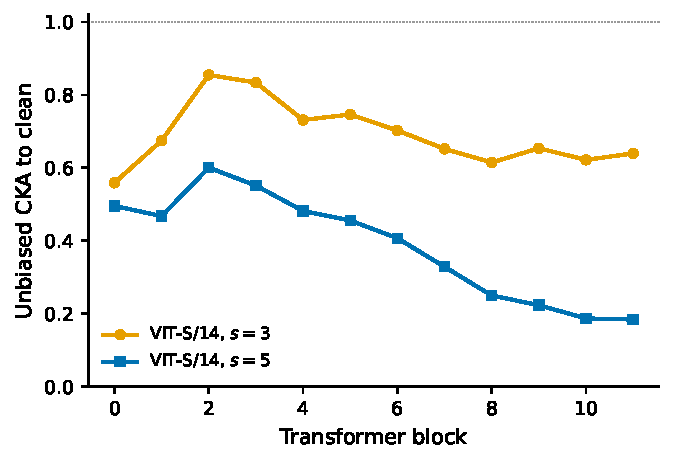
\includegraphics[width=\linewidth]{figures/fig_cka_depth.pdf}
\caption{CKA to clean by block: ViT-S/14 (solid) vs.\ ViT-B/14 (dashed,
severity 5). The drift gradient deepens with backbone size.}
\end{figure}

% ---------------------------------------------------------------------------
\section{Seed and Regularization Sensitivity}
\label{sup:sens}

The main curve regenerates across three split seeds ($\{42, 43, 44\}$)
crossed with three logistic-probe regularization strengths
($C \in \{0.1, 1, 10\}$) --- nine full re-runs of the ladder per severity.
\TableRef{sens} reports mean $\pm$ standard deviation. The regime structure
(never-negative grace, cliff, chance-level floor) is present in every
configuration; the cliff's exact position varies by at most one severity
step.

\begin{table}[h]
\centering\small
\caption{Accuracy (\%) across 3 split seeds $\times$ 3 probe-C values.}
\label{tab:sens}
\begin{tabular}{cc}
\toprule
Severity & Accuracy (mean $\pm$ std, $n$=9) \\
\midrule
0 & 92.2 $\pm$ 1.3 \\
1 & 93.6 $\pm$ 1.1 \\
2 & 89.4 $\pm$ 3.1 \\
3 & 67.3 $\pm$ 7.1 \\
4 & 27.2 $\pm$ 5.0 \\
5 & 10.9 $\pm$ 1.5 \\
\bottomrule
\end{tabular}

\end{table}

% ---------------------------------------------------------------------------
\section{Failure Analysis Detail}
\label{sup:failure}

\paragraph{Per-class death order.} \TableRef{failure} gives per-class
accuracy at severities 0/1/3/5. Automobile, cat, dog, and truck cross the
50\% line at severity 3; airplane, bird, deer, horse, and ship hold until
severity 4. Frog never crosses it --- the constant-class artifact analyzed in
the main text (\S6.4 there). Note also that the classes dying early
(automobile, truck) are exactly those whose clean embeddings sit closest to
their dark-counterpart embeddings in cosine terms, suggesting embedding
proximity, not semantic difficulty, governs the death order; we flag this as
an observation for the full-scale run to test, not a claim.

\begin{table}[h]
\centering\small
\caption{Per-class accuracy (\%) across the ladder.}
\label{tab:failure}
\begin{tabular}{lcccc}
\toprule
Class & Clean & Sev 1 & Sev 3 & Sev 5 (\%) \\
\midrule
airplane & 92 & 100 & 77 & 8 \\
automobile & 100 & 100 & 33 & 0 \\
bird & 100 & 100 & 56 & 0 \\
cat & 83 & 92 & 42 & 0 \\
deer & 91 & 100 & 64 & 0 \\
dog & 85 & 85 & 46 & 0 \\
frog & 92 & 92 & 92 & 100 \\
horse & 93 & 93 & 73 & 0 \\
ship & 100 & 100 & 62 & 0 \\
truck & 100 & 100 & 46 & 0 \\
\bottomrule
\end{tabular}

\end{table}

\paragraph{Persistence.} Every image misclassified at severity 1 remains
misclassified at severity 5 (100/100 on the pilot fold). A hundred
clean-correct images flip by severity 5.

\begin{figure}[h]
\centering
\includegraphics[width=\linewidth]{figures/failure_grid.png}
\caption{Clean-correct images misclassified at severity 5 (title shows the
dark prediction). Most dark predictions are ``frog'' --- the readout
collapse of the main text.}
\end{figure}

% ---------------------------------------------------------------------------
\section{Efficiency}
\label{sup:eff}

Latency measured on CPU (batch 1) with interleaved rounds to cancel
machine-contention drift: 4 rounds $\times$ 25 iterations per arm, median
per arm. Adapters add 21--25\% latency for at most 1.18M trainable
parameters.

\begin{table}[h]
\centering\small
\caption{Latency and throughput by arm.}
\label{tab:eff}
\begin{tabular}{lcccc}
\toprule
Arm & Backbone (M) & Trainable (M) & Latency (ms) & Acc (dark, \%) \\
\midrule
frozen_backbone & 22.1 & 0.00 & 42.8 & 56.3 \\
lora_r4 & 22.4 & 0.29 & 56.9 & -- \\
lora_r8 & 22.6 & 0.59 & 50.6 & -- \\
lora_r16 & 23.2 & 1.18 & 50.7 & -- \\
\bottomrule
\end{tabular}

\end{table}

% ---------------------------------------------------------------------------
\section{Prediction-Distribution Statistics}
\label{sup:collapse}

Per-severity statistics of the fixed probe's output distribution
(\TableRef{collapse}): top-1 predicted class and its share, number of
classes ever predicted, and Shannon entropy of the prediction distribution
normalized by $\ln 10$ (uniform $= 1.0$). The collapse to a constant class
at severity 5 (entropy 0.02, two classes used) is the mechanism behind
frog's spuriously perfect per-class accuracy.

\begin{table}[h]
\centering\small
\caption{Prediction-distribution statistics of the fixed probe by severity.}
\label{tab:collapse}
\begin{tabular}{cclcc}
\toprule
$s$ & top-1 class & share & classes used & $H/\ln 10$ \\
\midrule
0 & horse  & 0.12 & 10 & 0.99 \\
1 & horse  & 0.12 & 10 & 0.99 \\
2 & ship   & 0.12 & 10 & 0.99 \\
3 & frog   & 0.28 & 10 & 0.91 \\
4 & frog   & 0.72 & 10 & 0.50 \\
5 & frog   & 0.99 & 2  & 0.02 \\
\bottomrule
\end{tabular}
\end{table}

\end{document}
